\documentclass[openany, a4paper, 10pt]{article}
\usepackage{emptypage}
\usepackage{simple}
\usepackage{csquotes}
\usepackage{float}
\usepackage{graphicx}
\usepackage{tabularx}
\usepackage{adjustbox}
\usepackage{eurosym}
\usepackage{xcolor}
\usepackage{amsmath}
\usepackage{listings}
\newenvironment{vplace}[1][1]
  {\par\vspace*{\stretch{#1}}}
  {\vspace*{\stretch{1}}\par}

\begin{document}
\pagenumbering{roman}
\begin{titlepage}

\begin{figure}[htbp]
\flushright

\includegraphics[height=2cm]{img/log_uni}
\end{figure}

\begin{center}
\begin{vplace}
\begin{LARGE}
\textbf{Università degli Studi di Padova} \\
\end{LARGE}


\vspace{8pt}

\begin{Large}
\textsc{Dipartimento di Matematica "Tullio Levi-Civita"} \\
\end{Large}

\vspace{8pt}

\begin{large}
\textsc{Corso di Laurea in Informatica}\\
\end{large}

\vspace{110pt}
\begin{figure}[htbp]
\begin{center}

\includegraphics[width=\textwidth]{img/logo}
\end{center}
\end{figure}
\vspace{80pt}


\begin{center}
  \begin{huge}
\textbf{CrownSouls} \\
\end{huge}
\vspace{20pt}
\begin{LARGE}
Progetto di Programmazione ad Oggetti
\end{LARGE}
\end{center}


\vspace{80pt}

\begin{large}
Enrico Buratto \\
1142644
\end{large}

\end{vplace}

\line(1, 0){338} \\

\vspace{10pt}

\begin{normalsize}
\textsc{Anno Accademico 2019-2020}
\end{normalsize}

\end{center}
\end{titlepage}

%**************************************************************
% Indici
%**************************************************************
\cleardoublepage
\pdfbookmark{\contentsname}{tableofcontents}
\setcounter{tocdepth}{5}
\tableofcontents
\clearpage

\begingroup
    \let\clearpage\relax
    \let\cleardoublepage\relax
    \let\cleardoublepage\relax
\endgroup

\cleardoublepage

\setcounter{page}{1}
\pagenumbering{arabic}

%%%%%%%%%%%%%%%%%%%%%%%%%%%%%%
% DA REPLICARE PER OGNI FILE %
%     (un file a sezione)    %
%%%%%%%%%%%%%%%%%%%%%%%%%%%%%%

\newpage
\section{Introduzione}

\subsection{Abstract}
Si vuole realizzare un programma per la gestione di un inventario giocatore per il gioco \textit{Action RPG} "Dark Souls". Il giocatore possiede svariati elementi di diversi tipi; questi elementi possono infatti essere:
\begin{itemize}
  \begin{description}
    \item \textbf{Armature}: oggetti indossati dal giocatore per aumentare la resistenza al danno inflitto dai nemici;
    \item \textbf{Armi}: oggetti utilizzati dal giocatore per infliggere danno ai nemici;
    \item \textbf{Anelli}: oggetti utili al giocatore per l'aumento delle proprie statistiche; una volta indossati nel gioco, il giocatore vedrà aumentate alcune statistiche personali o delle armi;
    \item \textbf{Scudi}: oggetti utilizzati dal giocatore per ridurre il danno dai colpi nemici;
    \item \textbf{Guanti}: oggetti utilizzati sia come armatura, poiché aumentano la resistenza al danno, sia come arma, poiché permettono di infliggere danno;
    \item \textbf{Scudi d'attacco}: oggetti utilizzati sia come scudo, poiché riducono il danno dai colpi nemici, sia come arma, poiché permettono di infliggere danno.
  \end{description}
\end{itemize}

Un inventario è composto da un insieme di oggetti appartenenti alle diverse tipologie; ogni oggetto presente nell'inventario possiede delle caratteristiche tecniche proprie della categoria di appartenenza. \\
Il programma deve poter simulare un inventario di questo tipo, permettendo l'inserimento, la rimozione, la modifica e la visualizzazione degli oggetti e delle loro proprietà.


\subsection{Funzionalità}
Per facilitare la visualizzazione degli oggetti dell'inventario, questi sono suddivisi all'interno del programma in quattro diverse schede; ogni scheda rappresenta una sottosezione dell'inventario, e mostra al suo interno solo gli elementi appartenenti alla categoria indicata dal titolo.\\
Per la gestione degli oggetti dell'inventario sono presenti le seguenti funzionalità:
\begin{itemize}
  \item Caricamento ed esportazione dell'intero inventario da e su file \texttt{.xml};
  \item Aggiunta di un nuovo oggetto all'inventario;
  \item Modifica di un elemento già presente nell'inventario;
  \item Rimozione di un elemento dell'inventario;
  \item Rimozione di tutti gli elementi presenti;
  \item Visualizzazione di oggetti dell'inventario divisi per categoria di appartenenza;
  \item Visualizzazione delle caratteristiche di ogni elemento dell'inventario, comprese alcune statistiche calcolate automaticamente dal programma;
  \item Visualizzazione di avvisi d'errore.
\end{itemize}

\section{Breve manuale}
Brevissimo manuale d'uso del programma

\section{Progettazione}
Lo sviluppo del progetto si è basato sul pattern \textbf{Model-View} di \textit{Qt} e metodologia mista \textit{top-down} e \textit{bottom-up}. \\
Oltre alla gerarchia, è stato realizzato un Container templatizzato per il contenimento degli oggetti appartenenti alla gerarchia.
Sono stati realizzati inoltre:
\begin{itemize}
  \item Una GUI (Graphical User Interface), basata su classi preesistenti di Qt;
  \item Un Model, il quale si occupa della gestione dei dati del programma, basato anch'esso su classi preesistenti di Qt;
  \item Un filter proxy, che funge da intermediario tra model e view e permette di filtrare i dati per la visualizzazione corretta su ogni tab;
  \item Una classe di Input/Output su file XML.
\end{itemize}

\begin{figure}[H]
  \centering
  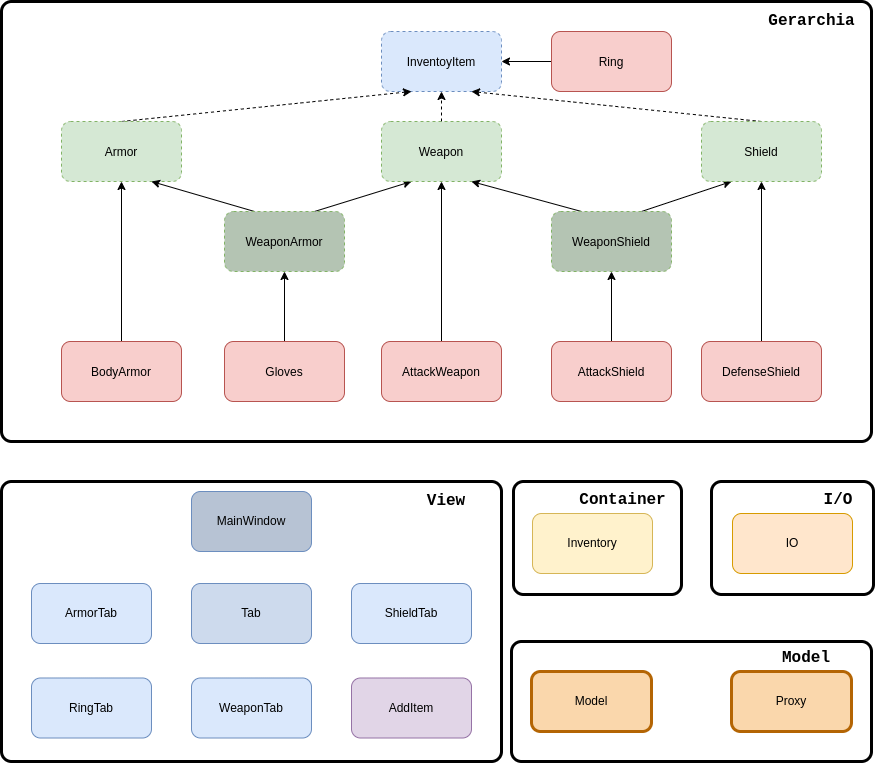
\includegraphics[width = \linewidth]{img/diagramma}
  \caption{Diagramma delle classi di CrownSouls.}
\end{figure}

\subsection{Gerarchia}
La gerarchia è composta dalla classe base astratta \textit{InventoryItem}, dalla quale deriva \textbf{direttamente} la classe concreta \textit{Ring} e \textbf{virtualmente} le classi astratte \textit{Armor}, \textit{Weapon} e \textit{Shield}. Da queste tre classi derivano \textbf{singolarmente} e \textbf{direttamente} le tre rispettive classi concrete \textit{BodyArmor}, \textit{AttackWeapon} e \textit{DefenseShield}. Viene inoltre utilizzata l'\textit{ereditarietà multipla} per la definizione di classi che rappresentano oggetti appartenenti a più tipi; nello specifico, la classe \textit{WeaponArmor} deriva direttamente da \textit{Armor} e \textit{Weapon}, e la classe \textit{WeaponShield} deriva direttamente da \textit{Weapon} e \textit{Shield}. Questa forma di ereditarietà multipla è di tipo \textbf{is-a}, poiché un oggetto WeaponArmor è sia un oggetto Weapon che un oggetto Armor (e lo stesso vale per WeaponShield). Da queste due classi astratte derivano poi rispettivamente le classi concrete \textit{Gloves} e \textit{AttackShield}. \\
Ciascuna classe implementa dei metodi virtuali che riguardano l'impostazione e il recupero delle diverse proprietà degli elementi, e dei metodi virtuali specifici di ogni sottoclasse astratta per il calcolo e l'ottenimento di statistiche basate sulle proprietà. L'utilizzo del polimorfismo in tale contesto viene illustrato in seguito.

\subsection{Container}
È stata implementata una classe \textit{Inventory} che funge da container. La classe fornisce un template di smart pointer, e simula una lista singolarmente linkata con alcuni accorgimenti: a differenza di una lista singolarmente linkata standard, infatti, essa fornisce anche un puntatore all'ultimo elemento, e permette l'accesso diretto in sola lettura a un dato elemento tramite l'overloading dell'operatore accesso agli elementi del puntatore ([]). \\
La classe \textit{Inventory} contiene al suo interno due classi annidate:
\begin{itemize}
  \item La classe \textit{SmartP} rappresenta uno smart pointer; è infatti questa classe a rappresentare un elemento del container di tipo T templatizzato. Oltre al contenuto effettivo dell'elemento e al puntatore all'elemento successivo, la classe è fornita anche di:
  \begin{itemize}
    \item Costruttore e costruttore di copia profondo;
    \item Distruttore profondo;
    \item Assegnazione profonda;
    \item Overloading degli operatori dereferenziazione e accesso a membro;
    \item Overloading degli operatori booleani uguaglianza e disuguaglianza.
  \end{itemize}
  \item La classe \textit{Iterator} rappresenta l'iteratore del container. Nello specifico, un oggetto di classe Iterator è un iteratore costante, poiché non permette il side effect degli oggetti a cui punta. Questa classe presenta l'overloading dei seguenti operatori:
  \begin{itemize}
    \item Incremento prefisso;
    \item Dereferenziazione;
    \item Accesso a membro;
    \item Uguaglianza e disuguaglianza.
  \end{itemize}
\end{itemize}
La classe container fornisce diverse funzionalità di inserimento, cancellazione e ricerca; essa infatti permette:
\begin{itemize}
  \item L'inserimento e la rimozione di oggetti in testa, in coda o in una posizione data;
  \item La modifica di un oggetto a una posizione data (sovrascrittura);
  \item La lettura di oggetti in testa, in coda o a in una posizione data grazie all'overloading dell'operatore [].
\end{itemize}

\subsection{Modello}
Modello

\subsection{GUI}
GUI

\subsection{I/O}
Il programma permette la lettura e la scrittura di interi inventari. Questa possibilità è data dalla classe \textit{IO}, la quale fornisce i metodi necessari all'input e all'output dei dati tramite file .xml. Questi metodi risolvono il problema specifico del programma sviluppato, e non sono pertanto applicabili ad altri problemi.

\subsection{Polimorfismo}
Polimorfismo

\subsection{Scelte progettuali}
\begin{itemize}
\item Si è scelto di utilizzare una lista singolarmente linkata per la facilità e l'efficacia di questa struttura dati in un problema come quello in oggetto. Sono stati però seguiti degli accorgimenti per la semplificazione dell'accesso in sola lettura dati (tramite operatore []) e per la diminuzione dello sforzo computazionale. Un esempio di questo è la presenza di un puntatore all'ultimo elemento, che permette la riduzione di alcune operazioni, tra cui l'aggiunta e la rimozione in coda, da tempo O(n) a tempo costante;
\item Si è scelto di optare per una classe di Input/Output non scalabile per questioni di tempo. Una classe facilmente adattabile a più problemi, infatti, avrebbe richiesto uno studio più approfondito e un utilizzo pesante di polimorfismo sulla gerarchia; questo è certamente auspicabile, ma purtroppo incompatibile con le tempistiche reali del progetto.
\end{itemize}

\section{Gestione di Progetto}

\subsection{Suddivisione del lavoro progettuale}
Il progetto è stato iniziato all'inizio del mese di giugno e si è concluso il giorno precedente alla consegna (4 luglio 2020).\\
Il progetto, nella la sua completezza ha richiesto circa \textbf{110} ore equalmente divise tra i due componenti del gruppo, che sono:
\begin{itemize}
    \item Buratto Enrico - 1142644
    \item Ostanello Emanuele - 1143439
\end{itemize}
Entrambi i componenti hanno contribuito a tutte le parti del progetto; la progettazione iniziale dei diversi componenti del progetto è stata concepita in totale collaborazione tramite la piattaforma di comunicazione vocale \textit{Discord}, necessaria nel periodo di distanziamento sociale che si è sovrapposto a buona parte del periodo di progettazione e sviluppo. Tuttavia, i singoli componenti hanno approfondito maggiormente un determinato ambito di progetto; nello specifico:
\begin{table}[H]
\begin{center}
\begin{tabular}{c|c}
\textbf{Enrico Buratto}        & \textbf{Emanuele Ostanello} \\ \hline
Codifica Gerarchia e Container & Apprendimento Qt            \\
Codifica Model                 & Codifica View              
\end{tabular}
\end{center}
\end{table}

\subsection{Timeline individuale}
Il lavoro individuale ha richiesto circa \textbf{55 ore} sulle 50 ore previste; le ore in eccesso sono dovute principalmente alla difficoltà di comunicazione a distanza, dovuta al periodo attuale. Nonostante questo, si può dire che il carico di lavoro è stato ben calibrato in base alla disponibilità oraria personale e a quanto sviluppato.
\begin{table}[H]
\begin{center}
\begin{tabular}{l|c}
\textbf{Fasi progettuali}        & \textbf{Ore utilizzate} \\ \hline
Analisi del problema             & 5                       \\
Progettazione                    & 13                      \\
Apprendimento Qt                 & 4                       \\
Codifica e implementazione Model & 17                      \\
Codifica e implementazione View  & 4                       \\
Test e Debug                     & 8                       \\
Relazione                        & 4                       \\ \hline
\textbf{Ore totali}              & \textbf{55}            
\end{tabular}
\end{center}
\end{table}

\subsection{Ambiente di lavoro}
Il progetto è stato sviluppato con \texti{Qt Creator v4.11.2} e \textif{Atom v1.47.0} su sistema operativo \textit{Arch Linux}; il compilatore usato è stato \textit{gcc v10.1.0}. Essendo il compilatore e la versione di \textit{Qt} del sistema di sviluppo più aggiornati rispetto alle specifiche, sono stati effettuati frequenti allineamenti con la macchina virtuale, contenente \textit{Ubuntu 18.04 LTS} con \textit{gcc v7.4.0} e \textit{Qt} alla versione v5.9.5. Questo ha permesso di verificare la compatibilità di quanto prodotto con le specifiche tecniche richieste.

\subsection{Istruzioni di compilazione ed esecuzione}
Il progetto prevede la compilazione tramite file .pro e tool qmake. Le istruzioni per la compilazione e l'esecuzione sono quindi le seguenti:
\begin{center}
\centering
\begin{verbatim}
  $ qmake CrownSouls.pro
  $ make
  $ ./CrownSouls
\end{verbatim}
\end{center}

Viene inoltre fornito un file \texttt{.xml}, locato nella cartella \texttt{extra}, contenente un inventario precompilato di prova.

\subsection{Considerazioni finali}
Il progetto ha richiesto un modesto impegno, soprattutto per quanto riguarda la progettazione e l'organizzazione del lavoro, avvenute a distanza. Una volta che il gruppo si è organizzato e il lavoro è stato diviso, però, lo sviluppo è stato abbastanza lineare, costante nel tempo e senza particolari complicazioni. \\
Entrambi i componenti del gruppo hanno utilizzato una parte considerevole di tempo per l'apprendimento e l'implementazione del \textit{proxy model}, che inizialmente ha dato non pochi problemi. Una volta risolti questi, però, lo sviluppo è continuato velocemente. \\
Concludendo, possiamo affermare che il progetto è stato abbastanza lungo e impegnativo, ma lo studio individuale e la scrittura di codice "reale" ha portato i suoi frutti.

\end{document}
